

%!TEX root = /Users/daniel/Documents/thesis/thesis.tex
\chapter{Erkennung handgeschriebener Symbole}

% (fold)
\label{cha:erkennung}

Die Erkennung handgeschriebener Symbole ist das Herzstück von Detexify. Hier wird einer unbekannten Eingabe von Daten ein \LaTeX-Symbol zugeordnet.
% Genau genommen wird der Eingabe eine Rangfolge von Symbolen zugeordnet, welche in der in \ref{sub:symbolsuche} beschriebenen Liste auftaucht, nachdem ein Nutzer ein Symbol gezeichnet hat.

Im Zentrum jeder Mustererkennungsaufgabe steht dabei der Erkennungsalgorithmus (\ref{sec:klassifizierung}). Je nach verwendetem Verfahren geht dem eine Vorverarbeitung (\ref{sec:vorverarbeitung}) und Merkmalsextraktion (\ref{sec:merkmale}) voraus. In diesem Kapitel stelle ich ich Möglichkeiten vor und analysiere sie auf ihre Tauglichkeit für Detexify.

\section{Terminologie}

% (fold)
\label{sec:terminologie}

Wie in jedem Forschungsgebiet hat sich auch bei der Handschrifterkennung eine Nomenklatur entwickelt, die die verschiedenen Aspekte des Themas beschreibt.

Man unterscheidet zwischen \emph{Online}- und \emph{Offline}-Systemen \cite{Tappert:1990p10302}. Bei Online-Systemen wird die Erkennung durchgeführt während der Nutzer schreibt. Die Striche werden dabei vom Eingabegerät (häufig ein Grafiktablett, in Detexify i.d.R. eine Computermaus) als Funktion \( t \mapsto \alpha \), wobei \( \alpha \) den Zustand der Stiftspitze kodiert, an das System übertragen. Das heißt, es stehen für die Erkennung alle dynamischen Eigenschaften des Geschriebenen zur Verfügung, wie die Anzahl, Reihenfolge und Richtung der einzelnen Pinselstriche. Im Gegensatz dazu verarbeiten Offline-Systeme Scans von Geschriebenem, arbeiten also zu einem Zeitpunkt, wenn der Schreibvorgang längst beendet ist. Sie können also außer Pixeln keine weiteren Informationen verwenden. Detexify ist ein Online-System.

Der Zustand der Stiftspitze besteht in Online-Systemen in der Regel aus den Koordinaten $(x,y)$, der Information, ob die Spitze das Tablett berührt, oft bezeichnet mit \emph{pen-up} bzw. \emph{pen-down} und in manchen Fällen auch aus der Neigung und dem Azimut.

Aus den Daten werden dann häufig Merkmale abgeleitet, sog. \emph{Features}. Man unterscheidet zwischen \emph{globalen} und \emph{lokalen} Features \cite{Tapia:2007p9160}. Lokale Features sind solche, die von einzelnen Punkten auf einem Strich und dessen benachbarten Punkten abgeleitet werden. Globale Features werden hingegen von der Menge der Striche als Ganzes abgeleitet.

\section[Herausforderungen]{Herausforderungen der Erkennung von \LaTeX-Symbolen}\label{sec:herausforderungen} Die Erkennung von handgemalten \LaTeX-Symbolen ist allein durch die enorme Anzahl der Symbole eine große Herausforderung \cite{Koerich:2003p1562}. Hinzu kommt, dass die Symbole aus sehr unterschiedlichen Alphabeten kommen. Es kommen lateinische, griechische, mathematische und weitere Symbole vor. Im Gegensatz zu asiatischen Sprachen, die ebenfalls sehr große Alphabete aufweisen\footnote{In Japan werden heute 6000-7000 Buchstaben verwendet. In China ist die Anzahl der im täglichen Leben verwendeten Buchstaben bei etwa 5000 \cite{Jaeger:2003p1097}}, ist jedoch die Anzahl und Reihenfolge der Striche nicht vorgegeben, was die Erkennung zusätzlich verkompliziert \cite{Watt:2005p1816}. Außerdem gibt es sehr viele sehr ähnliche Symbole wie $\rightarrow,\mapsto,\leadsto,\rightharpoonup,\hookrightarrow,\rightarrowtail$. Dazu kommen noch die Probleme vor der jede Handschrifterkennung steht, wie unterschiedliche Schreibstile sowohl von unterschiedlichen Schreibern als auch natürliche Variationen in der Schreibweise eines Einzelnen.

In Detexify wird diese Variation noch zusätzlich erhöht, da in den meisten Fällen eine herkömmliche Computermaus zum zeichnen der Symbole Verwendung findet, statt ein Grafiktablett, das eine gewohnte Stiftführung ermöglicht.

Ein guter Klassifizierungsalgorithmus muss also einiges leisten um der Situation gerecht zu werden.

\section{Eingabe} \label{sec:input}

Die Eingabe erfolgt für Handschrifterkennungssysteme häufig durch ein Grafiktablett. Dies ist auch in Detexify eine Möglichkeit, aber nicht die Regel. Die in \ref{sub:symbolsuche} beschriebene Zeichenfläche erlaubt sowohl die Eingabe über ein Grafiktablett als auch per Maus, wobei letzteres jeder Computeranwender zuhause hat. Die Eingabe erfolgt in der Webanwendung und die Daten, die an Server gesendet werden und damit den Erkennungsalgorithmus erreichen sind durch das \ac{REST}-Interface (siehe \ref{subsub:erkennung}) spezifiziert. Die Daten bestehen aus einer Liste von Strichen, wobei jeder Strich aus einzelnen Punkten, die die Bewegung der Stiftspitze beschreiben, besteht. Ein Punkt beinhaltet seine Koordinaten $x$ und $y$ sowie einen Zeitstempel $t$. Im \ac{JSON}-Format sieht das wiefolgt aus:

\lstinline![[{"x":125.5, "y":219.133331298828, "t":1269620535913}, ...], [...]]!

\section{Vorverarbeitung und Normalisierung I}
\label{sec:vorverarbeitung}

Eine Vorverarbeitung (Preprocessing) der Daten bevor sie an die Erkennungsalgorithmen ausgeliefert werden, ist eine wirksame Methode um Rauschen, das z.B. durch Ungenauigkeiten der Eingabegeräte oder Unachtsamkeit des Schreibers, entstehen kann, zu relativieren. Vorverarbeitung kann aber auch überflüssige Informationen entfernen, die vom Erkennungsalgorithmus nicht verwendet werden. Zudem kann durch Normalisierung der Daten ungewollte Variation reduziert werden. Es gibt kaum ein System zu Handschrifterkennung, das keine Vorverarbeitung durchführt \cite{Jaeger:2003p1097,Plamondon:2000p10303,Tappert:1990p10302}.

Die Auswahl der Maßnahmen hängt natürlich auch vom ausgewählten Erkennungsalgorithmus ab und aus diesem Grund werden die in Detexify angewandten Maßnahmen auch hier noch nicht erläutert, sondern erst in \ref{sec:vorverarbeitung2}, nach der der Analyse der Erkennungsalgorithmen. Da aber die Vorverarbeitung ein wichtiger Schritt ist, der schon vor der Klassifikation stattfindet, möchte ich hier bereits darauf hinweisen.

% section preprocessing_und_normalisierung (end)
\section{Merkmale} \label{sec:merkmale}

Merkmale sind (häufig numerische) Werte, die aus den Mustern extrahiert werden, die in der Regel in einem Vektor, dem Merkmalsvektor, zusammengefasst werden. Der Vektorraum in dem diese Vektoren liegen heißt dann der Merkmalsraum. Das in Detexify verwendete Verfahren erfordert keine Merkmalsextraktion. Der Merkmalsraum ist direkt der Raum der Pinselstriche.

\section{Klassifizierung}

% (fold)
\label{sec:klassifizierung}

Die Klassifizierung ist in der Mustererkennung der Vorgang unbekannten Daten eine Klasse zuzuordnen. Im Fall von Detexify ist dies ein \LaTeX-Symbol. Sie kann auf unterschiedliche Weisen erfolgen.

Zur Erkennung einzelner handgeschriebener Symbole wurden bereits unterschiedlichste Klassifikationsverfahren verwendet \cite{Plamondon:2000p10303}. Um ein leistungsstarkes Backend für Detexify zu entwickeln musste also ein Verfahren ausgewählt und gegebenenfalls optimiert werden, dass den spezifischen Anforderungen der Anwendung und der Architektur gerecht wurde.

Die Anforderungen sind die folgenden:
\begin{description}
  \label{desc:anforderungen}
  \item[Adaptionsfähigkeit] Es sollte jeder Zeit ein Training zusätzlicher Symbole möglich sein.
  \item[Skalierbarkeit] Die Erkennungsraten sollten auch bei einer großen Anzahl von Klassen gut sein.
  \item[Laufzeitverhalten] Das Laufzeitverhalten sollte eine Erkennung in Echtzeit ermöglichen.
  \item[Interaktivität] Es sollten die besten $N$ Symbole zur Auswahl angezeigt werden.
\end{description}

Ein besonderes Interesse galt in meinem Fall natürlichen den Verfahren, die für Symbolerkennung, insbesondere mathematischer Symbole, bereits erfolgreich eingesetzt wurden. Dabei handelt es sich um \ac{SVM}, \ac{HMM} und \ac{DTW}. Es gibt auch einige wenige Strukturelle Ansätze.

\subsection{Strukturelle Methoden} \label{sub:strukturelle_methoden}

Strukturelle Methoden basieren auf der Annahme, dass Handschrift aus elementaren Formen, auch Allographen genannt, besteht. Die Darstellung einer Klasse erfolgt dann als strukturelle Repräsentation (z.B. als Baum oder Graph) bestehend aus diesen Allomorphen. Die Vorgehensweise lässt sich am besten an einem Beispiel illustrieren. \citet{Fitzgerald:2004p10858} stellen mathematische Symbole als eine Kombination von Merkmalen der Typen \emph{Linie}, \emph{C-Form} oder \emph{O-Form} dar. Diese Merkmale werden mithilfe von Fuzzylogik aus den Strichen extrahiert und zur Zuordnung des richtigen Labels kommt wieder Fuzzylogik zum Einsatz. Dabei haben sie für jede Symbolklasse, die sie verwenden, eine eigene Fuzzy-Regel erstellt. Im zitierten Artikel waren das Regeln für die Zahlen 1-9 und kleingeschriebene lateinische Buchstaben. Es ist offensichtlich, dass ein solches Vorgehen für Detexify mit nahezu 1000 Symbolklassen nicht in Frage kommen kann. Zum Problem für jede Klasse ein Modell zu definieren kommt hinzu, dass das System nicht \emph{adaptionsfähig} im in \ref{desc:anforderungen} definierten Sinne ist, da jedes neue Symbol ein neues Modell braucht. Ohnehin ist es schwierig bei einer so großen Anzahl von Symbolklassen eine gemeinsame Struktur zu finden, die einen Strukturellen Ansatz praktikabel macht. Aus den genannten Gründen habe ich Strukturelle Methoden als ungeeignet für Detexify verworfen.

\subsection{Künstliche Neuronale Netze} \label{sub:kuenstliche_neuronale_netze}

Neuronale Netze haben bekanntlich Schwierigkeiten, wenn die Anzahl der Klassen groß ist \cite{Jaeger:2003p1097}. Dementsprechend ist die Anzahl der in Übersichtsartikeln zur Erknennung von Mathematischen Formeln wie \cite{Chan:2000p559} und \cite{Tapia:2007p9160} zitierten Arbeiten, die neuronale Netze verwenden, äußerst gering und ich habe keinen nach 1996 veröffentlichten Artikel gefunden, der Neuronale Netze für diese Aufgabe verwendet. Neuronale Netze können also als irrelevant abgehakt werden.

\subsection[SVM]{SVM - Support Vector Machines} \label{sub:svm}

\ac{SVM}s \cite{kernels} haben sich zu einem beliebten Klassifikationsverfahren für bestimmte Problemklassen entwickelt. Bei dem Verfahren betrachtet man eine Menge von (Trainings-)Objekten in einem Verktorraum (dem Merkmalsraum). Jedes Objekt gehört einer Klasse an und nun legt man eine Hyperebene so durch den Raum, dass die Klassen getrennt und der Rand zu beiden Seiten der Hyperebene maximal wird. Das Verfahren ist natürlich nur sinnvoll, wenn sich die Klassen linear trennen lassen. Ist dies nicht der Fall, bedient man sich des Kernel-Tricks \cite[S.15]{kernels} um den Merkmalsraum auf einen höherdimensionalen Verktorraum abbilden, in dem die Klassen linear trennbar sind.

\ac{SVM}s sind binäre Klassifizierer. Um sie also bei $N>2$ Klassen verwenden zu können gibt es unterschiedliche Strategien. Zum einen gibt es die \ac{WTA}-Strategie bei der $N$ binäre Klassifizierer konstruiert werden, wobei der $i$-te Klassifizierer $\rho_i$ die Klasse $C_i$ und $C_i^{\complement}$ (also alle anderen Klassen) unterscheidet. Einem unbekannten Objekt $x$ wird dann die Klasse zugeordnet, deren SVM $\rho_i$ das beste Ergebnis zurückliefert\footnote{Eine SVM ist als Funktion realisiert, die die Lage eines Eingabevektors zur Hyperebene zurückgibt. Das Ergebnis ist besser wenn der Eingabevektor weit auf der richtigen Seite liegt, also der Abstand zur Ebene größer ist.}. Zum anderen gibt es die \ac{MWV}-Strategie bei der für jedes Paar von Klassen $C_i$ und $C_j$ ein Klassifizierer $\rho_{ij}$ mit den Objekten aus $C_i$ gegen die Objekte aus $C_j$ trainiert wird. Für ein unbekanntes Objekt $x$ werden nun alle $N(N-1)/2$ Klassifizierer nach ihrer Stimme gefragt und die Klasse mit den meisten Stimmen gewinnt. Weitere Kombinationsstrategien finden sich in \cite{Duan:2005p11426} und \cite{Platt:2000p11488}.

\citet{Tapia:2003p11202,Tapia:2005p11236} verwenden \ac{DAGSVM}s \cite{Platt:2000p11488} zur Symbolerkennung in einem System, dass u.a. mathematische Formeln auf einer Elektronischen Tafel erkennt.
\citet{Golubitsky:2009p2456,Keshari:2008p528,Golubitsky:2009p2321} stellen Mathematische Symbole als Merkmalsvektor bestehend aus der Koeffizienten einer Funktionalapproximation der Striche dar und trainieren damit \ac{SVM}s, die sie mit \ac{MWV} kombinieren. Die genannten Autoren berichten auch von guten Ergebnissen — jedoch hätten \ac{SVM}s für Detexify einen entscheidenden Nachteil.

Das Hauptproblem besteht darin, dass SVMs schlecht nachtrainiert werden können. Um nachträglich ein neues Trainingsmuster hinzuzufügen, müssen bei $N$ Klassen beim deutlich besseren MWV-Verfahren \cite{Duan:2005p11426} $N-1$ SVMs angepasst (das heißt die Hyperebenen neu ausgerechnet) werden. Um eine neue Klasse hinzuzufügen müssen ebenfalls $N$ neue SVMs eingefügt werden. Ein inkrementelles Training ist also bei SVMs gar nicht denkbar. SVMs sind also ebenfalls nicht \emph{adaptionsfähig} und kommen daher nicht wirklich in Frage.

\subsection[HMM]{HMM - Hidden Markov Models} \label{sub:hmm}

\ac{HMM} sind ein statistisches Mustererkennungsverfahren, das schon seit langem in der Spracherkennung eingesetzt wird \cite{Rabiner:1989p11574}. Das liegt daran, dass es besonders geeignet ist zeitliche Muster zu modellieren und außerdem Segmentierung und Klassifizierung integriert \cite{Kosmala:1998p11691}. Der Merkmalsvektor darf dabei von Muster zu Muster in der Länge variieren.
Dabei beschreibt ein HMM einen diskreten Markovprozess $q=(q_t)_{t=0,1.\dots}$ dessen Zustandsfolge aber nicht sichtbar (also verborgen, daher der Name) ist. Stattdessen sieht der Beobachter eine Symbolfolge $\mathbf{O}=O_1\dots O_T, O_t\in V$ aus einem endlichen Alphabet $V=\{v_i\}_{i=1\dots K}$ wobei zu jedem Zeitpunkt $t$ jeweils $O_t$ nur vom verborgenen Zustand $q_t$ der diskreten Markovkette abhängt. Abb.~\ref{fig:hmm} illustriert das Modell. Eine ausführliche Einführung zu HMMs inklusive Erklärung von diskreten Markovprozessen findet sich bei \citet{Rabiner:1989p11574}.

\begin{figure}[htbp]
  \centering 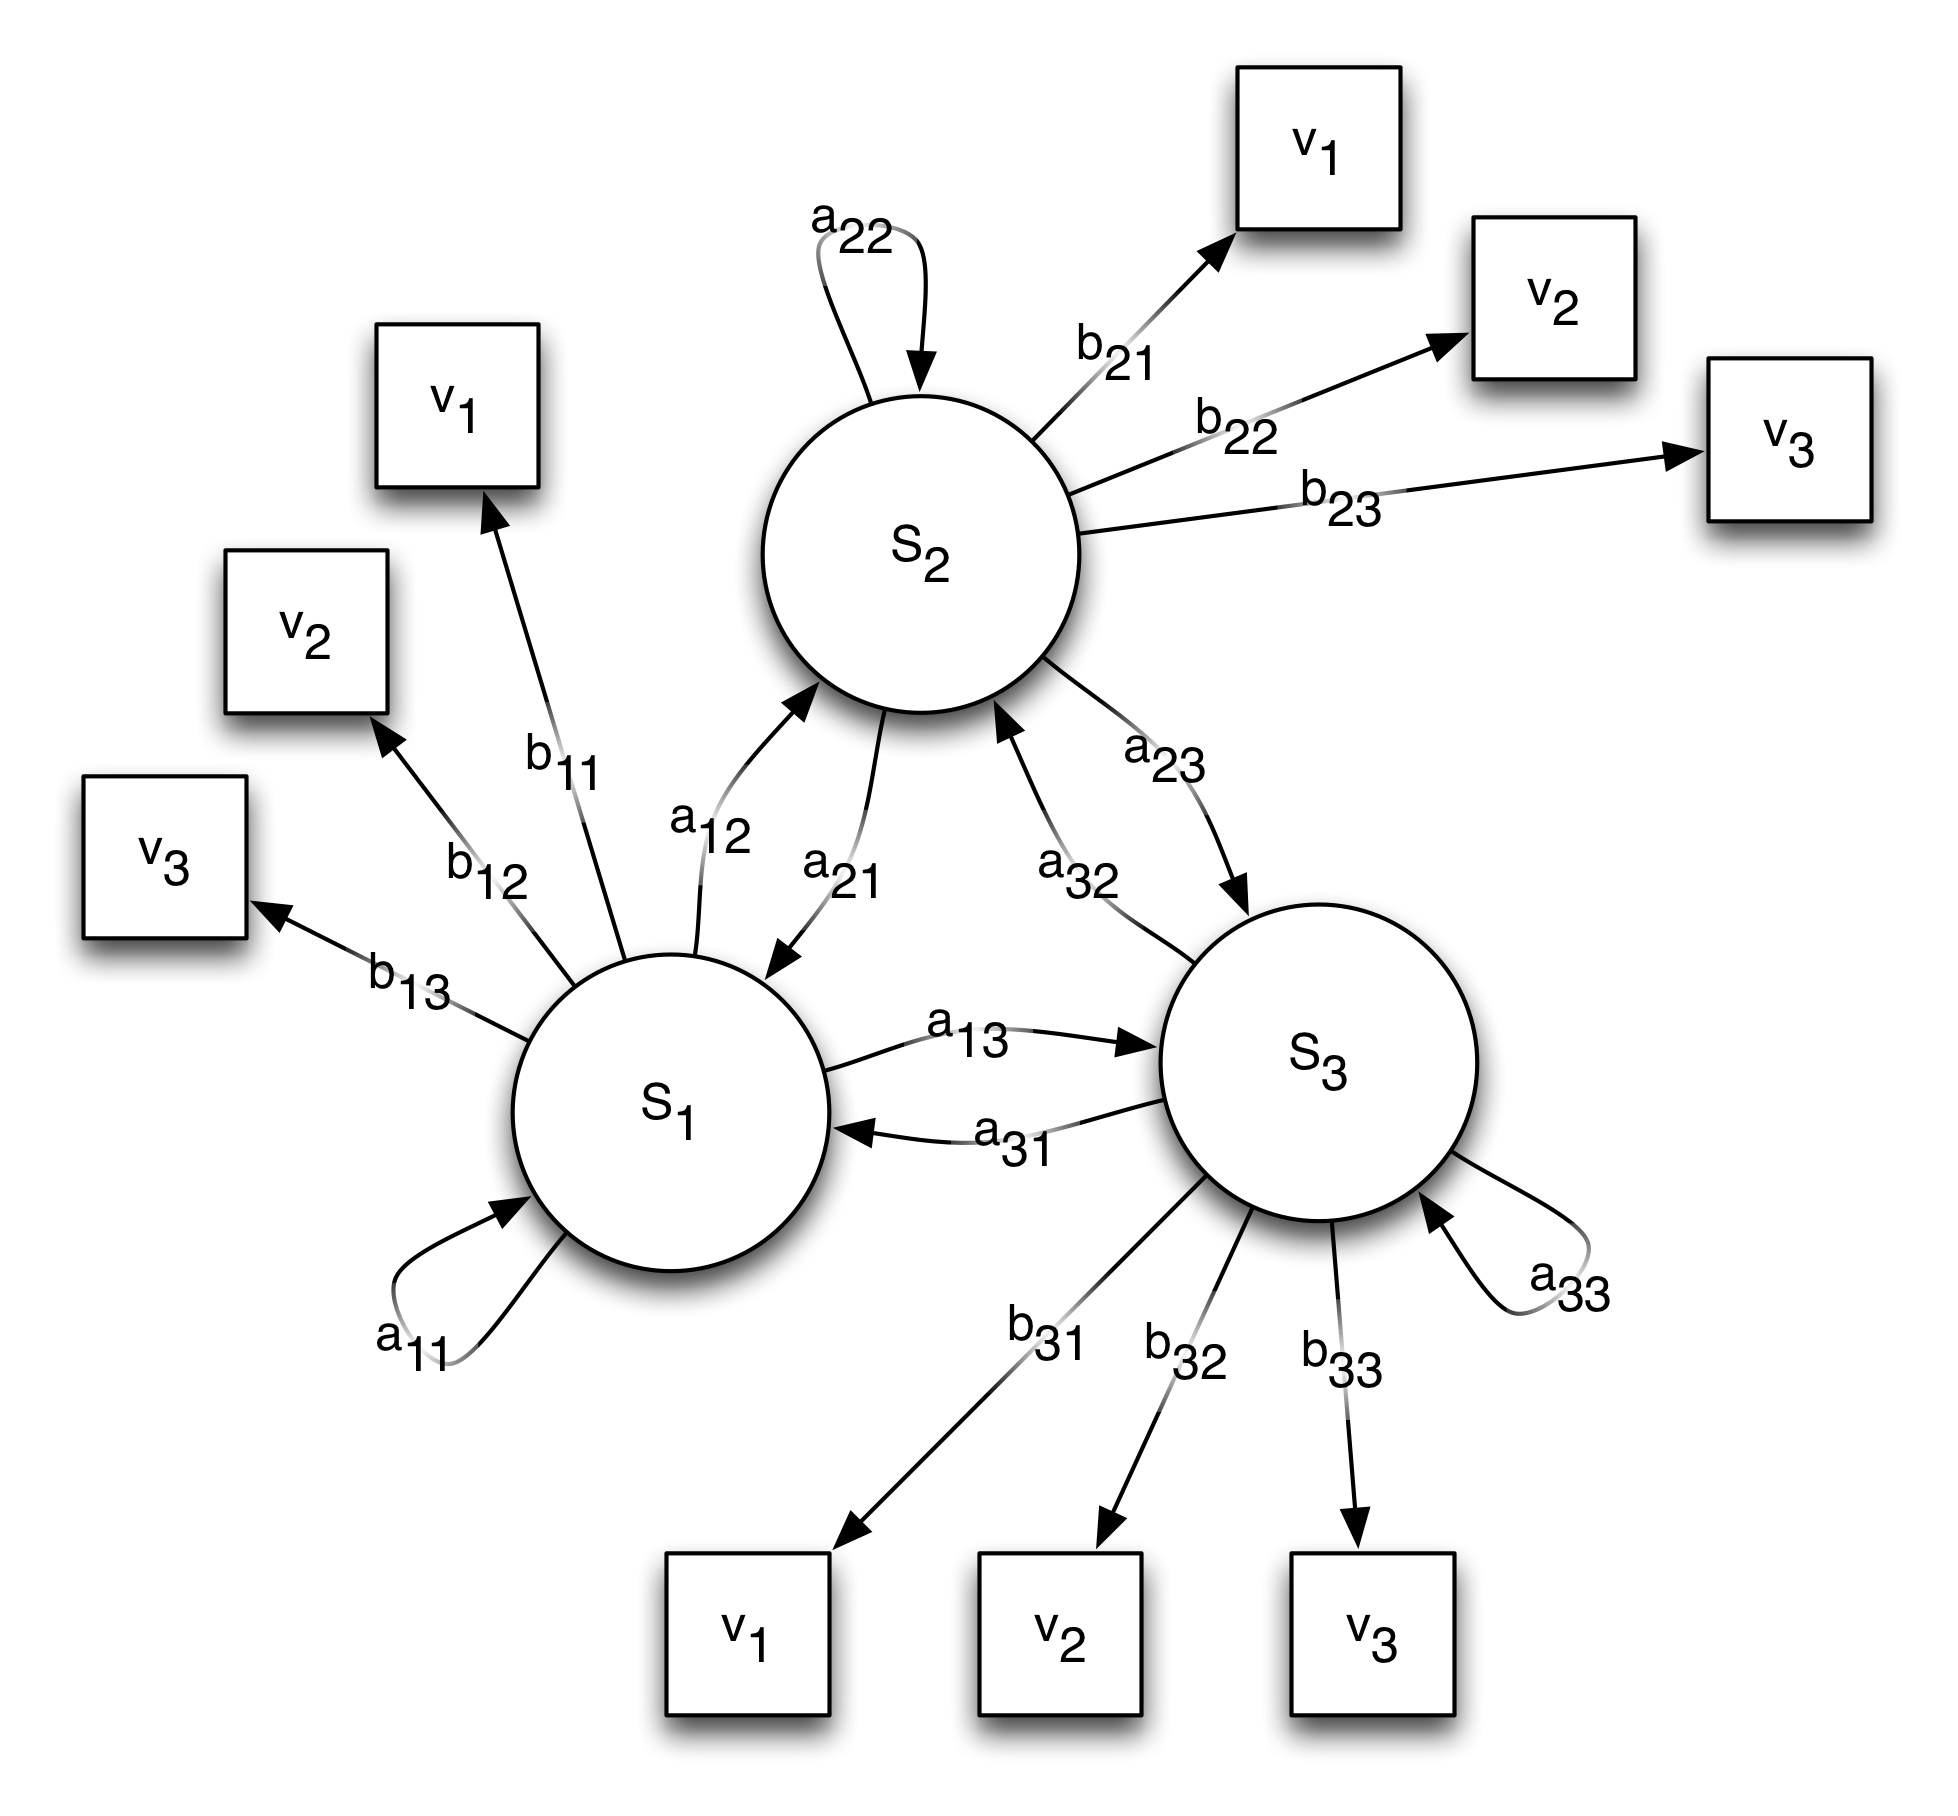
\includegraphics[width=\textwidth]{figures/hmm.png}
  \caption{HMM}
  \label{fig:hmm}
\end{figure}

Man verwendet eine HMM dann folgendermaßen: Jede Klasse $C_i$ bekommt eine HMM $\lambda_i$ deren Parameter anhand einer Stichprobe trainiert werden. Einem unbekannten Objekt, das als Folge $\mathbf{O}$ von Merkmalsvektoren beobachtet wird, wird dann die Klasse zugeordnet, für die die Wahrscheinlichkeit $P_{\lambda_i}(\mathbf{O})$, dass die Folge von der zugehörigen HMM erzeugt wurde, maximiert wird.

\citet{Xie:2007p11427} beschreibt ein System zur Erkennung mathematischer Symbole, das auf HMM basiert. In derselben Arbeit wird auch ein Klassifizierer, der auf DTW basiert vorgestellt, und für diesen werden beeindruckende Erkennungsraten von im besten Fall 94.8 \% angeben. Obwohl sich ein Vergleich angeboten hätte werden jedoch für das HMM-basierte System keine absoluten Erkennungsraten vorgestellt, sondern lediglich relative Veränderungen, wenn mit den Parametern der HMM gespielt wird. Das stimmt etwas nachdenklich.

\citet{Winkler:1996p11716} kombiniert mehrere HMMs, die mit unterschiedlichen Merkmalen trainiert werden, und erreicht bei einem Alphabet von 84 Symbolen im besten Fall eine Erkennungsrate von 91 \%.

Von der Leistungsfähigkeit her scheinen HMMs also durchaus eine Option für Detexify zu sein. Ein Problem ergibt sich aber wieder bei der \emph{Adaptionsfähigkeit}: Die Effektivität eines HMM hängt von seiner Modellierung ab (Anzahl der Zustände, Übergangswahrscheinlichkeiten, Ausgabewahrscheinlichkeiten) und diese müssten idealerweise für jede Symbolklasse individuell optimiert werden \cite{Fitzgerald:2005p331}. Das Hinzufügen einer neuen Symbolklasse umfasst also die Definition eines neuen HMMs und dessen Training.

\subsection{Nächste-Nachbarn-Klassifikation} \label{sub:knn}

Der $k$-nächste-Nachbarn-Algorithmus \cite[S.18]{eva:pattern} ist eines der einfachsten Verfahren um einem unbekannten Muster eine Klasse zuzuweisen. Dazu werden als Training einfach Vertreter der Klassen in einem Merkmalsraum gespeichert. Einem unbekannten Muster wird dann durch ein Mehrheitsvotum der $k$ nächsten Nachbarn eine Klasse zugeordnet. Darum wird diese Art der Klassifikation auch häufig \emph{template matching} genannt. Eine zentrale Rolle nimmt dabei das Abstandsmaß, das die Nachbarschaft bestimmt, ein \cite{Jaeger:2003p1097}. Es beeinflusst die Güte der Klassifikation, aber auch durch seine Laufzeitkomplexität den zeitlichen Aufwand des Vorgangs.

Dabei ist Nächste-Nachbarn-Klassifikation besonders bei Problemen beliebt, in denen die Anzahl an Klassen sehr hoch ist, wie beispielsweise bei japanischen Schriftzeichen \cite{Jaeger:2003p1097}. Eine Analyse zur Eignung für Detexify scheint also angebracht.
% Laut Jiang Script Kapitel 4 ist KNN mit vielen Trainingsdaten nahezu so gut wie Bayes (optimal)
% \citet{Tappert:1990p10302} sagt bei Online-Erkennung reichen wegen der Interaktivität einfachere Methoden, was bei mir ja voll zutrifft.

Die Bedingung der \emph{Adaptionsfähigkeit}, die ich in \ref{sec:klassifizierung} gefordert hatte, die bei den bisher vorgestellten Verfahren schwierig umzusetzen war, ist dabei bei der Nächste-Nachbarn-Klassifikation auf natürliche Weise dadurch gegeben, dass neue Trainingsmuster einfach nur gespeichert werden müssen. \emph{Interaktivität} kann leicht realisiert werden, indem jeder Klasse ein auf dem Abstandsmaß basierender Wert zugewiesen wird. So erhält man für ein unbekanntes Muster eine Rangfolge der Klassen.

Es ist also zu klären, ob es ein Abstandsmaß gibt, das die Bedingungen \emph{Skalierbarkeit} und \emph{Laufzeitkomplexität} miteinander vereinen kann.

\subsection[DTW]{DTW - Dynamic time warping}

Ein vielversprechendes Abstandsmaß wurde bereits in \ref{sub:hmm} erwähnt. Es wird \emph{dynamic time warping} oder auch \emph{elastic matching} genannt. Es wurde bereits erfolgreich für lateinische und chinesische Schriftzeihen eingesetzt \cite{Tappert:1990p10302}. \citet{Xie:2007p11427} erreicht damit für die Erkennung mathematischer Symbole eine Erkennungsrate von 94.8 \%. Auch \citet{Golubitsky:2009p2433} bemerken:
% In diesem Paper gibts auch Infos zum verwendete Datensatz. Weitere Statistiken zu Elastic matching Parametern.
\begin{quote}
  Among the distance measures used for classifying handwritten mathematical symbols, the elastic matching distance is known to be one of the most accurate.
\end{quote}

\citet{Golubitsky:2009p1842} vergleichen DTW mit einem eigenen Abstandsmaß, das zwar deutlich schneller zu berechnen ist, aber auch 1-1,5\% schlechtere Erkennungsraten liefert. \citet{Labahn:2008p10301} kombinieren DTW mit weiteren Methoden in einem System, das die handschriftliche Eingabe von Formeln in ein \ac{CAS} ermöglicht.
Auch \citet{Vuong:2010p10279} verwenden DTW % mit Steigung und Krümmung
zu Erkennung mathematischer Symbole in einer erst kürzlich veröffentlichten Arbeit zum Thema Web-basiertes CAS mit handschriftlicher Eingabe. Es ist auffällig, dass gerade aktuellere Arbeiten DTW einsetzen. Obwohl das Verfahren schon so lange bekannt ist \cite{Tappert:1982p10305}, ist es immer noch konkurrenzfähig.

Aus diesen Gründen ist die Wahl für die Klassifikation in Detexify auf Nächste-Nachbarn-Klassifikation mit DTW als Abstandsmaß gefallen. Damit war die Aufgabe also den Algorithmus so zu implementieren und zu optimieren, dass die Bedingungen \emph{Skalierbarkeit} und \emph{Laufzeitkomplexität} erfüllt sind.

\section{Vorverarbeitung und Normalisierung II}
\label{sec:vorverarbeitung2}

Mit der Festlegung auf Nächste-Nachbarn-Klassifikation mit DTW als Abstandsmaß, können auch die notwendigen Maßnahmen zur Vorverarbeitung und Normalisierung der Striche erläutert werden. Es sind die folgenden:

\begin{description}
  \item[Normalisierung der Größe und Position]
  Die ankommenden Striche werden verschoben und skaliert, so dass sie unter Beibehaltung ihres Seitenverhältnisses\footnote{Der Erhaltung des Seitenverhältnisses ist sehr wichtig. Dies musste ich feststellen, als mir in der Haskell-Implementierung etwa 4-5\% Erkennungsrate fehlte, obwohl ich dachte, ich hätte alles eins zu eins von Ruby portiert.} zentriert und maximal im Quadrat \([0,1]\times[0,1]\) liegen. Dieser Schritt ist notwendig um zwei Muster überhaupt sinnvoll mit DTW vergleichen zu können.
  \item[Glättung]
  Jeder Punkt eines Striches wird durch das arithmetische Mittel des Punktes und seiner beiden Nachbarpunkte ersetzt.
  \item[Äquidistante Verteilung] Da die Zeichenfläche im Browser in Detexify eine gewisse Abtastrate hat, die erstens Herstellerabhängig sein kann, und zweitens zeitabhängig ist, kann die Verteilung der Punkte auf den Strichen sehr ungleich sein. Daher werden die Punkte neu verteilt, so dass die Entfernung zwischen zwei je Punkten gleichmäßig groß ist. Die Anfangs- und Endpunkte von Strichen werden dabei erhalten. \citet{Golubitsky:2009p1842} geben an, dass eine Äquidistante Verteilung der Punkte bei Verwendung von DTW sogar die beste Wahl ist.
  \item[Dominante Punkte] Punkte mit geringer Krümmung tragen zur Charakteristik eines Striches nicht viel bei, daher werden sie herausgefiltert. Es wird ein Grenzwinkel $\alpha$ definiert und es bleiben die Punkte erhalten, an denen sich die Richtung des Striches um mehr als $\alpha$ ändert. Durch diese Reduktion in der Anzahl der Punkte wird außerdem DTW geringfügig beschleunigt.
  \item[Verkettung] Da \ac{DTW} zwei Zeitreihen vergleicht, werden die Striche miteinander verkettet, so dass das Abstandsmaß direkt angewendet werden kann.\footnote{Dies hört sich im ersten Moment naiv an, aber alle versuchten Alternativen haben bei der Erkennung schlechtere Ergebnisse, als diese einfache Methode geliefert.}
\end{description}

% Verwerfen von Strichen wenn mehr als 10 verschweige ich.

Es gibt noch zwei Maßnahmen, die in der Literatur auftauchen, aber in Detexify keine Verwendung finden:

\begin{description}
  \item[Sortierung der Striche] Wie in \ref{sec:herausforderungen} erwähnt ist die Reihenfolge der Striche bei Mathematischen Symbolen einer großen Variation unterlegen. \citet{Matasakis:1999p9465} schlägt eine kanonische Sortierung der Striche vor, die dieses Problem beheben soll.
  \item[Richtungskorrektur der Striche] Dasselbe Problem tritt bei der Zeichenrichtung der Striche auf. Auch hier hat \citet{Matasakis:1999p9465} eine kanonische Zeichenrichtung vorgeschlagen und dreht Striche gegebenenfalls um.
\end{description}

Die Alternative zu den oben genannten Verfahren ist, für jede mögliche Zeichenreihenfolge und -richtung, ein eigenes Modell anzulegen. Es ist klar, dass das bei Symbolen mit vielen Strichen zu sehr vielen Modellen führen würde. Da das Training in Detexify aber ohnehin durch die Nutzer durchgeführt wird, habe ich mich bei Detexify für den folgenden Weg entschieden.

Es wird keine Umsortierung oder Richtungsänderung vorgenommen. Stattdessen wird die Eigenschaft der Nächste-Nachbarn-Klassifikation ausgenutzt, dass die Muster ohnehin direkt gespeichert werden. Variationen in der Anzahl, Sortierung und Richtung der Striche werden bewusst in Kauf genommen. Bei der Suche nach der richtigen Klasse werden also automatisch verschiedene Variationen, eben die, die von vorherigen Benutzern eintrainiert wurden, durchsucht.\footnote{Tatsächlich haben einige Benchmarks, die ich in Kapitel \ref{cha:benchmarks} aber nicht aufführe, gezeigt, dass eine Sortierung der Striche nicht hilft. Sowohl eine Sortierung wie \citet{Matasakis:1999p9465} sie vorschlägt als auch nach anderen Kriterien haben der Erkennungsraten entweder nicht verändert oder leicht verschlechtert.}

Durch Umsortierung oder Richtungsänderung kann man nämlich auch genau die Probleme schaffen, die man eigentlich unterbinden wollte \cite{Matasakis:1999p9465}. Man schafft außerdem neue Parameter, die wieder optimiert werden müssen.

\section{DTW} % (fold)
\label{sec:dtw}

Im folgenden wird der klassische DTW-Algorithmus beschrieben und unterschiedliche Optimierungsmöglichkeiten werden diskutiert.

\subsection{Der klassische DTW-Algorithmus} % (fold)
\label{sub:dtw}

Seien zwei Folgen von Punkten
\begin{align}
  \label{eqn:a}
  A &= a_1, \dots, a_n \\
  \label{eqn:b}
  B &= b_1, \dots, b_m
\end{align}
in einem Raum \( S \ni a_i, b_i ~\forall~i \) und %die Menge von Abbildungen
% \begin{equation*}
%   \label{eqn:mappings}
%   F = \{f:\{1,\dots,n\} \rightarrow \{1,\dots,m\}, ~f~\text{surjektiv, monoton wachsend} \}
% \end{equation*}
\( \delta : S\times S \rightarrow \mathbb{R}_0^+ \) eine Kostenfunktion
gegeben. In der Regel sind \(A\) und \(B\) Folgen in einem metrischen Raum z.B. \(\mathbb{R}^n\) und \(\delta\) ist eine Metrik.
Betrachten wir nun \( n\times m\)-Matrix
\begin{equation} \label{eqn:matrix}
  M = (d_{i,j})_{i=1\dots n, j=1\dots m} ~\text{mit}~ d_{i,j} = \delta(a_i,b_j)
\end{equation}
, dann ist ein Warping-Pfad ein stetiger (im unten erläuterten Sinne) Pfad durch diese Matrix.

\begin{align}
  W = w_0,\dots,w_K \hspace{1cm} w_l = (i,j)_l
\end{align}

$K$ ist dabei die Länge des Warping-Pfads. Die Stetigkeit des Pfads unterliegt den folgenden Bedingungen:

\begin{description}
  \item[Randbedingung] \( w_1 = (1,1) \) und \( w_K = (n,m) \). Dadurch beginnt der Warping-Pfad in der linken unteren Ecke der Matrix und endet in der rechten oberen Ecke.
  \item[Stetigkeitbedingung] Gegeben \( w_k = (i,j) \) und \( w_{k-1} = (i',j') \) so muss gelten \( i-i' \leqslant 1 \) und \( j-j' \leqslant 1 \). Dadurch sind nur Schritte zu benachbarten Zellen (auch diagonal) erlaubt.
  \item[Monotoniebedingung] Gegeben \( w_k = (i,j) \) und \( w_{k-1} = (i',j') \) so muss gelten \( i-i' \geqslant 0 \) und \( j-j' \geqslant 0 \). Dadurch werden rückwärtige Schritte (nach links oder unten) verhindert.
\end{description}

Es gibt natürlich einige Pfade die diese Bedingungen erfüllen. Nennen wir die Menge dieser Pfade
\[ \mathcal{W}=\{W~\text{ist Warping-Pfad}\} \]
dann ist der DTW-Abstand definiert durch
\begin{equation}
  \label{eqn:dtw}
  DTW(A,B) = \min_{W \in \mathcal{W}}{\frac{\sum_{i=1}^K d_{w_i}}{K}}
\end{equation}
. Dabei ist \( d_{w_i} \) das entsprechende Element der Matrix \ref{eqn:matrix}.

Diese abstrakte Definition bedeutet anschaulich, dass die Punkte in den zwei Folgen einander elastisch zugeordnet werden können, wobei es einige Beschränkungen gibt. Der erste Punkt der ersten Folge wird immer dem ersten Punkt der zweiten Folge und der letzte Punkt der ersten Folge immer dem letzten Punkt der zweiten Folge zugeordnet werden. Dazwischen müssen die Punkte zwar in der richtigen Reihenfolge bleiben und es dürfen keine übersprungen werden, aber es sind Mehrfachzuordnungen erlaubt. Gesucht wird die Zuordnung, die den Abstand minimiert. Abbildung~\ref{fig:dtw} illustriert dies.

\begin{figure}
  \centering 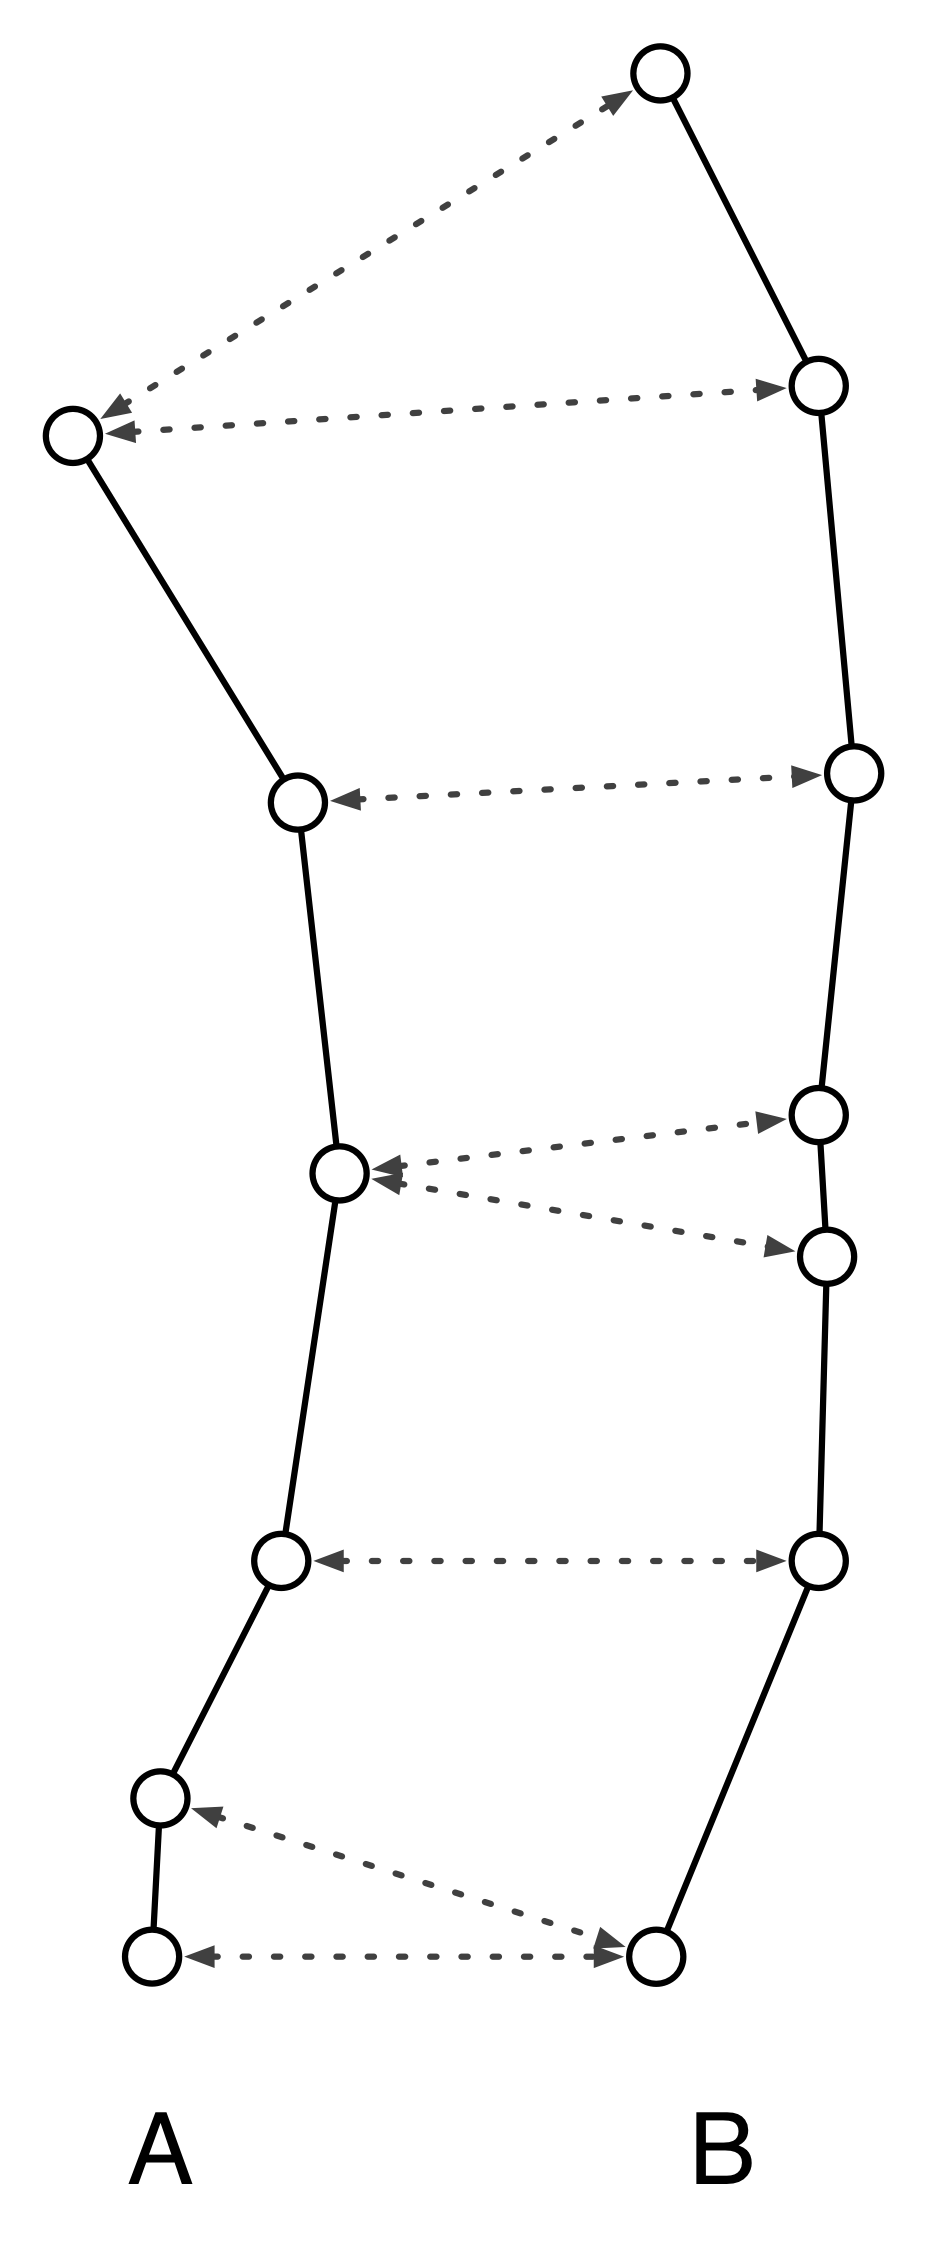
\includegraphics[width=4cm]{figures/dtw.png}
  \caption{Elastische Zuordnung bei DTW}
  \label{fig:dtw}
\end{figure}

Das gesuchte Minimum kann mithilfe von Dynamischer Programmierung \cite[S.323ff.]{algorithms} gefunden werden und zwar mithilfe der folgenden Rekurrenz:

\begin{equation}
  \label{eqn:dp}
  \gamma(i,j) =
  \begin{cases}
    \sum_{k=0}^j \delta(a_0, b_k) & i = 0 \\
    \sum_{k=0}^i \delta(a_k, b_0) & j = 0 \\
    \delta(a_i,~b_j) + \min\{~\gamma(i-1,j-1),~\gamma(i-1,j),~\gamma(i,j-1)~\} & \text{sonst}
  \end{cases}
\end{equation}

% dann ist
% \begin{equation}
%   \label{eqn:dpdtw}
%   DTW(A,B) = \frac{\gamma(n,m)}{K}
% \end{equation}.

In dieser Form hat DTW die Laufzeit- und Speicherplatzkomplexität \(\mathcal{O}(nm)\). Darum wundert es nicht, dass bereits einige Wissenschaftler versucht haben, den Algorithmus zu optimieren. Auch für Detexify ist dieses Laufzeitverhalten nicht ausreichend um eine Erkennung in Echtzeit zu ermöglichen.


\subsection{Beschränkung des Warping-Pfads} % (fold)
\label{sub:constrained_warping_window}

\begin{figure}
  \centering 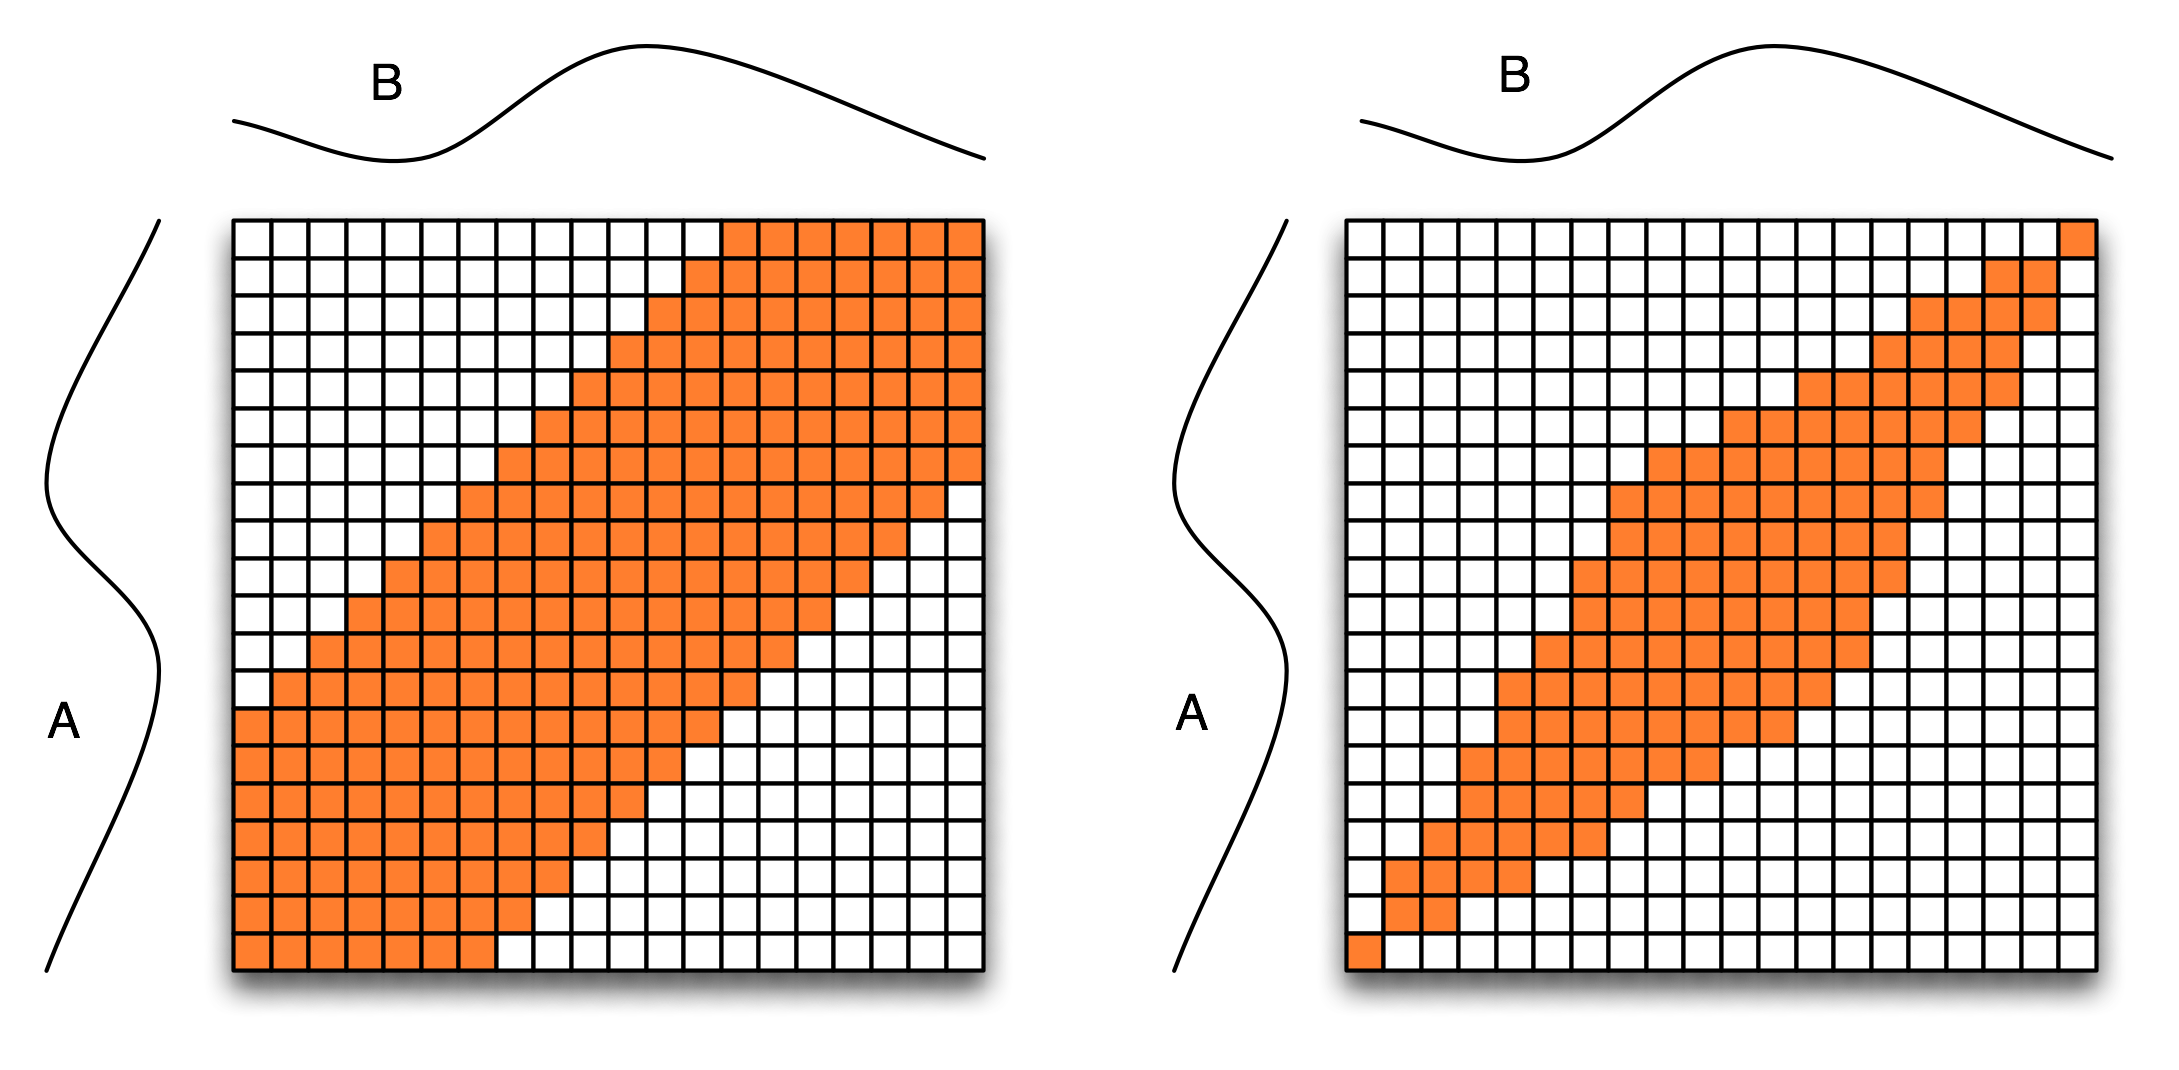
\includegraphics[width=\textwidth]{figures/constraints.png}
  \caption{Typische Beschränkungen das Warping-Pfades}
   Links: Sakoe-Chiba-Band, Rechts: Ikatura-Parallelogramm
  \label{fig:constraints}
\end{figure}


Es ist möglich DTW dadurch zu beschleunigen, dass bei der Suche nach dem optimalen Warping-Pfad nicht die ganze Matrix durchsucht wird. Stattdessen wird der Suchraum beschränkt. Abb.~\ref{fig:constraints} zeigt üblicherweise verwendete globale Beschränkungen. Es ist auch möglich lokale Beschränkungen wie in \cite{Rabiner:1993p11752} beschrieben festzulegen, \citet{Keogh:2005p7751} bemerken aber, dass das im Prinzip dasselbe, wie globale Beschränkungen sind, darum gehe ich darauf nicht näher ein. Nun könnte man glauben, dass sich eine solche Einschränkung nachteilig auswirkt. \citet{Ratanamahatana:2004p7522} berichten aber in ihrer Arbeit, dass eher das Gegenteil der Fall ist und Beschränkungen des Pfades sogar helfen, die Erkennungsraten zu verbessern. Dies kann dadurch verstanden werden, dass durch Beschränkungen pathologisches Warpen verhindert wird \cite{Keogh:2005p7751}.
%- Leichte Geschwindigkeitsverbesserung \( \mathcal{O}(ns) \) für fest gewähltes $s$
%- Sakoe and Chiba 1978 haben wohl schon rausgefunden, dass globale beschränkungen helfen \cite{Keogh:2005p7751}

Wenn beide Folgen die gleiche Länge $n$ haben, ist eine Möglichkeit den Warping-Pfad zu beschränken, einen Korridor um die Diagonale der Matrix festzulegen, aus dem nicht ausgebrochen werden darf. Beschrieben werden kann dies durch eine Beschränkung der Indizes des Warping-Pfades \( w_k = (i,j)_k \) und zwar gilt dann
\begin{equation}
  \label{eq:constraints}
  j - r(i) \leq i \leq j + r(i)
\end{equation}
, wobei $r(i)$ den erlaubten Korridor beschreibt.

Im Fall von \(r(i) = s\) also $r$ konstant reduziert sich damit die Komplexität von DTW von \( \mathcal{O}(n^2) \) auf \( \mathcal{O}(ns) \). Zusätzlich ermöglicht die Beschränkung bei fester Länge $n$ der Folgen eine weitere noch effektivere Optimierung:

\subsection{Untere Schranken} % (fold)
\label{sub:lower_bounding}

Gegeben ein Abstandsmaß \( \delta : S\times S \rightarrow \mathbb{R}_0^+ \) und eine untere Schranke \( \delta_{LB} \) d.h. \( \delta_{LB}(a,b) \leq \delta(a,b) ~\forall~ a,b \in S \), die deutlich günstiger zu berechnen ist, dann lässt sich mit dem folgenden naiven Algorithmus eine sequentielle Suche nach dem nächsten Nachbarn eines Elementes \( c \in S \) beschleunigen (vergl. \cite{Keogh:2005p7751}).

\begin{algorithm}
  \caption{Beschleunigung der Suche nach dem nächsten Nachbarn eines Elementes \(c\) durch eine untere Schranke}
  \begin{algorithmic}
    \STATE $\text{best\_so\_far} \gets \infty$
    \FORALL{samples $s$}
      \STATE $\text{lb\_dist} \gets \delta_{LB}(c,s)$
      \IF{$\text{lb} < \text{best\_so\_far}$}
        \STATE true\_dist $\gets \delta(c,s)$
        \IF{$\text{true\_dist} < \text{best\_so\_far}$}
          \STATE best\_so\_far $\gets$ true\_dist
          \STATE nearest\_neighbor $\gets s$
        \ENDIF
      \ENDIF
    \ENDFOR
  \end{algorithmic}
\end{algorithm}

Für DTW für Folgen derselben Länge $n$ mit reellen Messpunkten mit einer Beschränkung des Warping-Pfades der Form \ref{eq:constraints} haben \citet{Keogh:2005p7751} eine scharfe untere Schranke angegeben. Zudem haben \citet{Ratanamahatana:2004p7522} die Kritik entkräftet, dass vor der Verwendung einer solchen Optimierung eine lineare Interpolation der Folgen nötig ist, um sie auf dieselbe Länge zu bringen, und damit der Vorteil Folgen unterschiedlicher Länge vergleichen zu können verlogen ginge. Eine untere Schranke scheint also eine reizvolle Möglichkeit zu sein DTW zu beschleunigen.

%TODO wer hat vor \citet{Keogh:2005p7751} untere Schranken angegeben? Muss ich das erwähnen?

In Fall von Detexify sind die einzelnen Punkte der Folgen aber Punkte im \( \mathbb{R}^2 \) (siehe \ref{sec:vorverarbeitung}) und es ist intuitiv einzusehen, dass eine Reduktion auf eine Dimension einen zu hohen Informationsverlust nach sich ziehen würde. Es ist leider nicht leicht im  \( \mathbb{R}^2 \) auf eine zu \cite{Keogh:2005p7751} analoge Weise eine untere Schranke zu definieren, die sinnvoll einsetzbar ist.

\subsection{Eine untere Schranke für DTW für Folgen im \( \mathbb{R}^2 \)?}

\subsubsection{LB\_Keogh}
\label{ssub:lb_keogh}

Bevor ich das Problem im \( \mathbb{R}^2 \) erläutere, gebe ich noch eine kurze Erklärung der von \citet{Keogh:2005p7751} definierten unteren Schranke LB\_Keogh an.

Seien
\begin{align}
  Q &= q_1 \dots q_n  & q_i \in \mathbb{R} \\
  C &= c_1 \dots c_n  & c_i \in \mathbb{R}
\end{align}
zwei Folgen gleicher Länge $n$. \( \mathcal{W}_r \) sei die Menge der durch \(r\) beschränkten Warping-Pfade (siehe \ref{eq:constraints}). DTW sei (leicht verändert) gegeben durch
\begin{equation}
  \label{eq:keoghdtw}
  DTW(Q,C) = \min_{W \in \mathcal{W}_r}{\sqrt{\sum_{i=1}^n d_{w_i}}}
\end{equation}.
Mithilfe von \(r\) werden nun weitere Folgen $U$ und $L$ definiert:
\begin{align}
  U_i &= \max ~\{ q_{i-r}, \dots, q_{i+r} \}\\
  L_i &= \min ~\{ q_{i-r}, \dots, q_{i+r} \}
\end{align}
Es gilt offensichtlich
\begin{equation}
  \forall ~ i ~ U_i \geq q_i \geq L_i
\end{equation}.
Nun können wir eine untere Schranke für \ref{eq:keoghdtw} wiefolgt definieren:
\begin{equation}
  \label{eq:lbkeogh}
  \operatorname{LB\_Keogh}(Q,C) = \sqrt{\sum_{i=1}^n
  \begin{cases}
    \delta(c_i, U_i) & c_i > U_i \\
    \delta(c_i, L_i) & c_i < L_i \\
    0 & \text{sonst}
  \end{cases}
  }
\end{equation}

Die Intuition dahinter ist die folgende. Die Folgen $U$ und $L$ bilden eine Hülle um die ursprüngliche Folge $Q$. LB\_Keogh ist dann sozusagen der Abstand einer neuen Folge $C$ zu dieser Hülle (siehe Abbildung \ref{fig:lb_keogh}). Dass dies tatsächlich eine untere Schranke ist, haben \citet{Keogh:2005p7751} gezeigt. Sie argumentieren auch, dass ihre Schranke schärfer als die bisher in der Literatur aufgetauchten ist.

\begin{figure}
  \centering 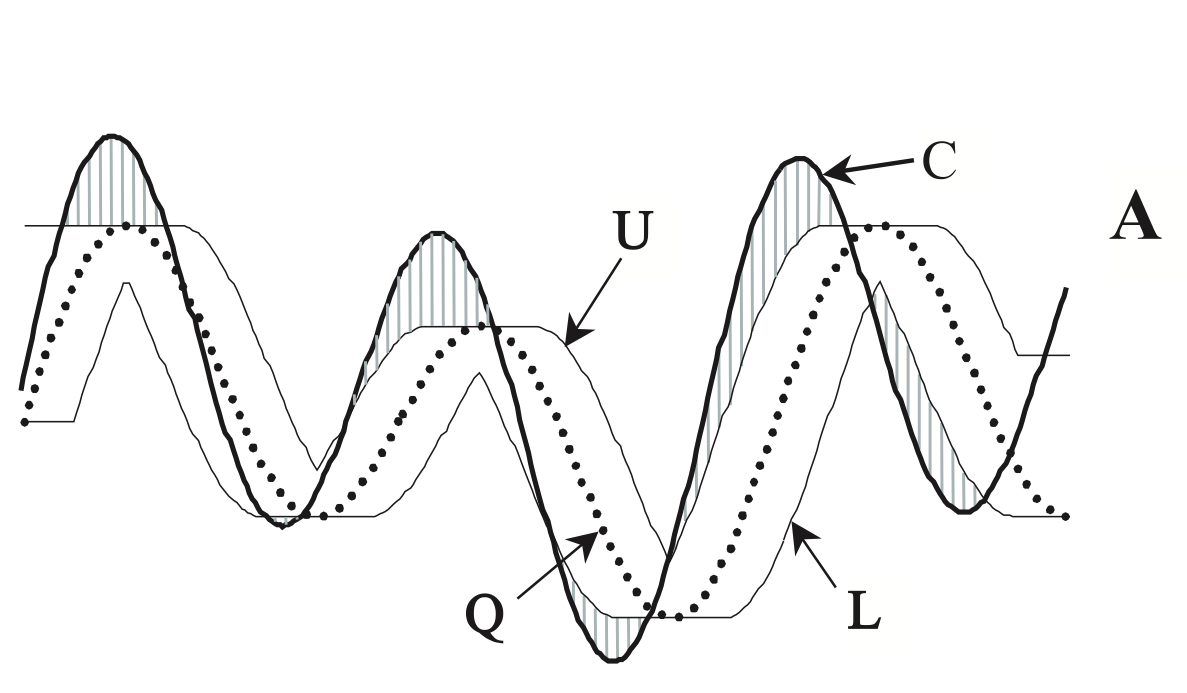
\includegraphics[width=10cm]{figures/lb-keogh.png}
  \caption{Grafische Darfstellung von LB\_Keogh. Grafik entnommen aus \cite{Keogh:2005p7751}}
  \label{fig:lb_keogh}
\end{figure}

\subsubsection{\(\mathbb{R}^2\)-analog zu LB\_Keogh}\label{subs:lb_keogh_analog}

Seinen nun zwei Folgen
\begin{align}
  A &= a_1 \dots a_n  & a_i \in \mathbb{R}^2 \\
  B &= b_1 \dots b_n  & b_i \in \mathbb{R}^2
\end{align}
gegeben.
\( \mathcal{W}_r \) sei wieder die Menge der durch \(r\) beschränkten Warping-Pfade. Wir definieren dann eine neue Folge $C$ durch
\begin{equation}
  C_i = \operatorname{conv} ~\{ a_{i-r}, \dots, a_{i+r} \}
\end{equation}
wobei
\[
  \operatorname{conv} X = \bigcap_{X\subseteq K \subseteq V \atop K\ \mathrm{konvex}} K
\]
die konvexe Hülle ist. Die neue Folge $C$ besteht also aus konvexen Polygonen. Für \ref{eq:keoghdtw} lässt sich nun eine untere Schranke wiefolgt definieren:
\begin{equation}
  \label{eq:lbkeoghanalog}
  \operatorname{LB}(A,B) = \sqrt{\sum_{i=1}^n
  \begin{cases}
    0 & b_i \in C_i \\
    \delta(b_i, C_i) & \text{sonst}
  \end{cases}
  }
\end{equation}
und dabei ist natürlich \( \delta(b_i, C_i) = \min\limits_{c \in C_i} \delta(b_i, c) \).

Das Problem besteht nun aber darin, dass diese untere Schranke nur dann effizient zu berechnen wäre, wenn beim Bilden der konvexen Hülle viele Punkte im inneren derselben liegen würden, denn die Komplexität der Berechnung des Abstandes zur konvexen Hülle ist proportional zur Anzahl der Ecken $v$. Es gilt zwar $v \leq r$ es ist völlig unklar wie stark $v$ typischerweise unter $r$ liegt. Geht man vor einer Gleichverteilung zwischen $2$ und $r$ aus so bleibt damit die Komplexität dieser unteren Schranke bei \( \mathcal{O}(rn) \) was der des ursprünglichen Algorithmus entspricht. Dadurch ist also nichts gewonnen. Aus diesem Grund entfällt auch der formale Beweis, dass es sich um eine untere Schranke handelt und es muss weiter nach praktikablen Optimierungen gesucht werden.
% subsubsection lower_bounding (end)

\subsection{Greedy Matching} % (fold)
\label{sec:greedy}

Es ist möglich DTW mit einem Greedy-Algorithmus \cite[S.370ff.]{algorithms} zu approximieren.

Grundsätzlich funktioniert eine Greedy-Approximation von DTW bei zwei Folgen $A$ und $B$ mit \(a_i,b_i \in S\) und einem Abstandsmaß \(\delta:S\times S \rightarrow \mathbb{R}_0^+\) folgendermaßen. Beginne mit den Startpunkten $a_1$ und $b_1$ ordne diese einander zu. Ordne dann jeweils die nächsten Punkte so einander zu, dass der Abstand unter \(\delta\) minimal ist (wähle das lokale Optimum). Wiederhole dies, bis in einer der beiden Folgen nur noch ein Punkt übrig ist. Ordne alle restlichen Punkte der anderen Folge diesem zu. Algorithmus \ref{alg:greedy} zeigt eine Implementierung in Pseudocode.
Wie man sieht hat der Algorithmus einen konstanten Speicherplatzaufwand und eine lineare Laufzeit.

\begin{algorithm}
  \caption{Greedy Matching}
  \label{alg:greedy}
  \begin{algorithmic}
    \STATE $a \gets \text{next from}~A$
    \STATE $b \gets \text{next from}~B$
    \STATE $d \gets \delta(a,b)$
    \STATE $a' \gets \text{next from}~A$
    \STATE $b' \gets \text{next from}~B$
    \WHILE{points left in $A$ $\wedge$ points left in $B$}
      \STATE $l, m, r \gets \delta(a',b), \delta(a', b'), \delta(a, b')$
      \STATE $\mu \gets \min ~\{l, m, r\}$
      %\COMMENT{ Important line }
      \STATE $d \gets d + \mu$
      \IF{$l = \mu$}
        \STATE $a \gets a'$
        \STATE $a' \gets \text{next from}~A$
      \ELSIF{$r = \mu$}
        \STATE $b \gets b'$
        \STATE $b' \gets \text{next from}~B$
      \ELSE
        \STATE $a \gets a'$
        \STATE $b \gets b'$
        \STATE $a' \gets \text{next from}~A$
        \STATE $b' \gets \text{next from}~B$
      \ENDIF
    \ENDWHILE
    \IF{no points left in $A$}
      \FORALL{points $p$ in $B$}
        \STATE $d \gets d + \delta(a',p)$
      \ENDFOR
    \ELSIF{no points left in $B$}
      \FORALL{points $p$ in $A$}
        \STATE $d \gets d + \delta(b',p)$
      \ENDFOR
    \ENDIF
  \end{algorithmic}
\end{algorithm}

\citet{MacLean:2010p9970} stellen eine Variante dieses Algorithmus vor. Sie verwenden ihn zur Erkennung mathematischer Symbole in Mathbrush, das in dieser Arbeit bereits erwähnt wurde (siehe auch \ref{sub:mathbrush} und \cite{Labahn:2008p10301}). Sie gehen bei der Zuordnung von Punkten aber simultan von beiden Seiten vor.
Welche Vorteile das gegenüber einer einseitigen Strategie bringt, erklären sie nicht. Sie vergleichen ihren Greedy-Algorithmus jedoch mit dem Standard-DTW-Algorithmus und kommen zum Ergebnis, dass der Greedy-Algorithmus zur Unterscheidung von mathematischen Symbolen ebenso geeignet ist. Insbesondere bei einer kleinen Anzahl von Punkten pro Strich (<30) ist der Greedy-Algorithmus sogar gleich gut geeignet und durch seine lineare Laufzeit natürlich wesentlich schneller. Bei ihren Tests verwenden sie 15796 handgeschriebene Symbole aus 70 Symbolklassen geschrieben von 20 unterschiedlichen Personen.

\subsection{Elimination}
\label{sec:elimnimation}

Eine weitere Optimierungsmöglichkeit besteht darin irrelevante Trainingsmuster im Suchraum zu eliminieren um für diese einen teuren DTW-Vergleich gar nicht mehr durchführen zu müssen. \citet{Watt:2005p1816} schlagen Elimination durch klassische Merkmale vor, d.h. es wird ein Merkmalsvektor gebildet und es wird nur noch für die besten $N$ Trainingsmuster, die auf Basis eines günstigen Abstandsmaßes gefunden werden, die DTW-Entfernung ausgerechnet. \citet{Watt:2005p1816} verlieren durch ein solches Verfahren 3\% an Erkennungsgenauigkeit aber vermeiden für fast 90\% des Suchraumes das teurere Abstandsmaß.
Ist das verwendete Abstandsmaß eine Metrik, so gibt es sogar exakte Eliminationsverfahren für die Nächste-Nachbarn-Klassifikation, die ohne Genauigkeitsverlust auskommen z.B. im $\mathcal{R}^2$ mithilfe von Voronoi-Diagrammen. DTW ist leider keine Metrik, darum bleiben mir solche Mittel verschlossen.
Aus diesem Grund werden Eliminationsverfahren in Detexify nicht zur Anwendung gebracht.
%TODO Vielleicht trotzdem mal Greedy-Algorithmus nach Hart (siehe Jiang-Script) testen?

\subsection{Parameter}
\label{sec:parameter}

Bei der Verwendung von template matching mit DTW als Abstandsmaß müssen einige Parameter festgelegt werden. Diese beeinflussen die Leistungsfähigkeit und Geschwindigkeit des Klassifikators und müssen sorgfältig ausgewählt werden. Die Parameter sind die folgenden:

\begin{description}
  \item[$n$] - Anzahl der Punkte pro Strich
  \item[$r$] - Fensterbreite bei beschränktem DTW (siehe \ref{eq:constraints})
  \item[$\delta$] - das verwendete innere Abstandsmaß (siehe \ref{sub:dtw})
  \item[$k$] - Anzahl der nächsten Nachbarn beim klassischen $k$-nächste-Nachbarn-Algorithmus
  \item[$C$] - Anzahl der Trainingsmuster pro Klasse
\end{description}

Da DTW schon häufig Verwendung gefunden hat, gibt es natürlich in der Literatur einige Angaben zu experimentell gefundenen Optima für bestimmte Parameter. Dabei ist natürlich zu bedenken, dass die optimale Parameterwahl immer vom konkreten Problem und natürlich auch von den Testdaten abhängt. Trotzdem bieten die Angaben gute Anhaltspunkte in welchen Bereichen sich sinnvolle Parameter bewegen.

\citet{Golubitsky:2009p1842} geben an, dass bei ihrer Konfiguration mit 107 Symbolklassen die Erkennungsrate mit Steigerung von $C$ fast linear ansteigt bis 25 Trainingsmuster pro Klasse erreicht sind. Ab dann sind die Zuwächse nicht mehr signifikant. Sie geben das Optimum für $n$ bei $k = 1$ mit $25$ an. Bei mehr Punkten fällt die Erkennungsrate sogar leicht. Sie haben auch mit $k$ experimentiert und kommen zum Schluss, dass bei kleinen Klassen ($C<10$) $k = 1$ am besten abschneidet. Werden die Klassen größer, so lohnen sich nach und nach immer größere Werte für $k$. Zum Beispiel ist für $C>25$  $k=5$ die beste Wahl. Der Vorsprung in der Erkennungsrate liegt aber bei weniger als 1\%.

\citet{Golubitsky:2009p2433} geben für $k=1$ und beschränkte Warping-Pfade die optimalen Parameter mit $n = 30$ und $r = 2$ an. Sie verwenden dabei quadratischen euklidischen Abstand als inneres Abstandsmaß $\delta$.

\citet{MacLean:2010p9970} verwenden in ihren Greedy-Variante von DTW ein Abstandsmaß, das auch die Steigung der Striche mit einbezieht, wie auch \citet{Tappert:1982p10305} es vorgeschlagen hat.
\citet{Vuong:2010p10279} Gehen noch einen Schritt weiter und verwenden sogar die Krümmung der Striche.